\documentclass[12pt, a4paper]{article}
    
\usepackage{homework}
\usepackage{amsmath}				% For Math
\usepackage{fancyhdr}				% For fancy header/footer
\usepackage{graphicx}				% For including figure/image
\usepackage{cancel}					% To use the slash to cancel out stuff in work
\usepackage{multirow}
\usepackage{lastpage}
\PassOptionsToPackage{hidelinks}{hyperref}
\usepackage{hyperref}    % For PDF metadata and links

% Set PDF metadata
\hypersetup{
    pdftitle={CENG4120 VLSI CAD Assignment 3 - Part B},
    pdfauthor={Yu Ching Hei},
    pdfsubject={CENG4120 Assignment},
    pdfkeywords={VLSI, CAD, Assignment},
    pdfcreator={LaTeX},
    pdfproducer={pdfLaTeX},
    pdflang={en-US},
    % bookmarks=false,
    bookmarksopen=false,
    bookmarksnumbered=false,
    colorlinks=false,
    pdfstartview={FitH}
    % pdfpagemode=UseOutlines
}

%%%%%%%%%%%%%%%%%%%%%%
% Set up fancy header/footer
\pagestyle{fancy}
\setlength{\headheight}{35pt}
\fancyhead[LO,L]{Name: Yu Ching Hei\\Student ID: 1155193237\\email: chyu2@cse.cuhk.edu.hk}
\fancyhead[CO,C]{}
\fancyhead[RO,R]{CENG4120 - VLSI CAD\\Assignment 3 - Part B\\Date: \today}
\fancyfoot[LO,L]{}
\fancyfoot[CO,C]{}
\fancyfoot[RO,R]{Page \thepage\ of \pageref{LastPage}}
\renewcommand{\headrulewidth}{0.4pt}
\renewcommand{\footrulewidth}{0.4pt}
%%%%%%%%%%%%%%%%%%%%%%

\begin{document}

\setcounter{section}{1}

\begin{enumerate}[label=\arabic*.]
    \item 
    \begin{description}
        \item[DRC Violation:] 0
        \item[Total Area:] 258.115 $\mu m^2$
        \item[Total Power:] 2.33769348 $mW$
        \item[Slack:] 0.031 $ns$
    \end{description}
    \item 263.7466 $\mu m^2$
    \item total area unchanged, while slack reduced to 0.024 $ns$ with increasing row density. 
    Total area unchanged probably because of the power routing, 
    and slack decreased because of the reduced separation between standard cells. 
    \item 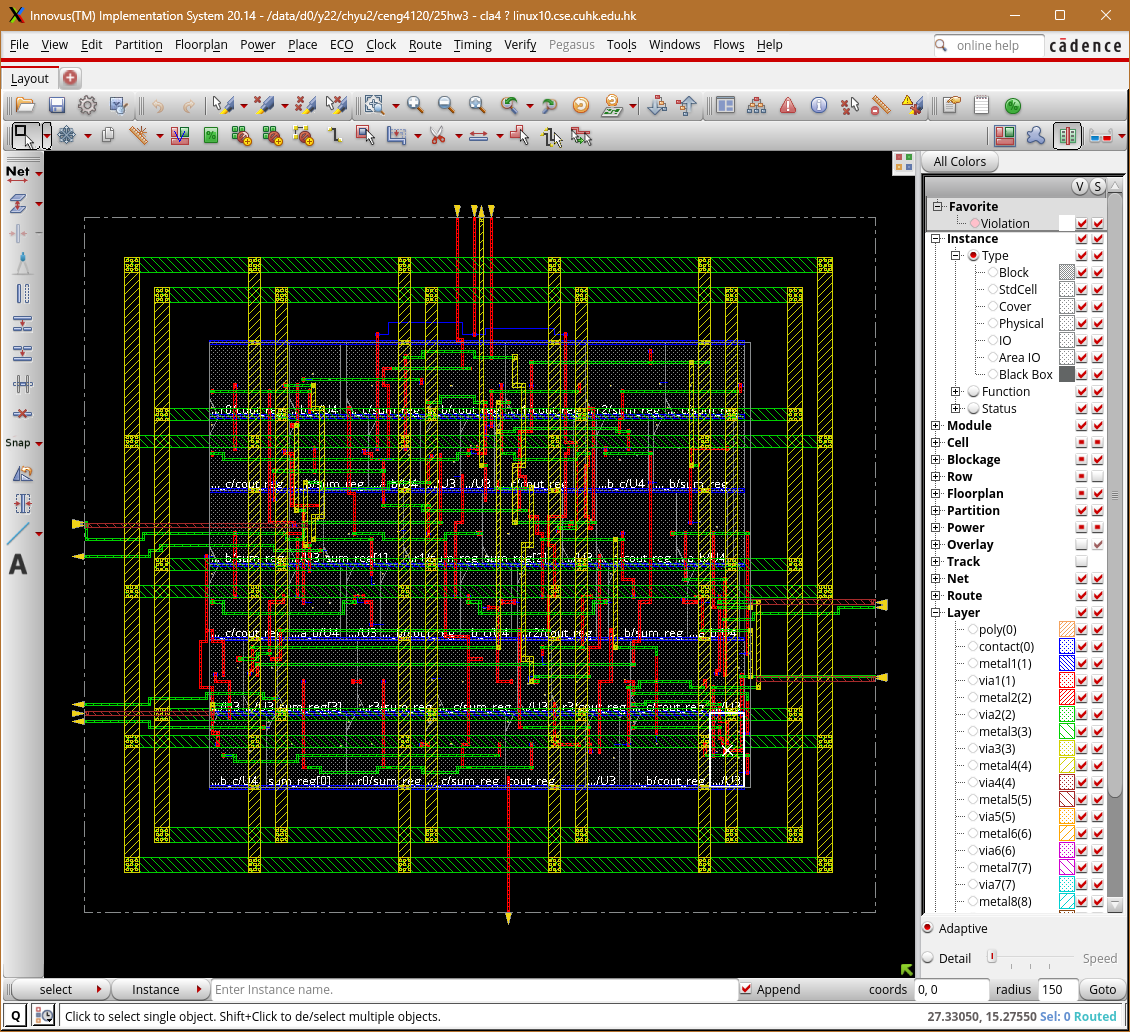
\includegraphics[width=0.9\textwidth]{figs/image.png}
\end{enumerate}
\end{document}